\section{Step 1 --- Image to Patch Tokens}

\textbf{Patch Partitioning and Linear Projection.}
The raw radiograph $X \in \mathbb{R}^{B \times 3 \times 224 \times 224}$ is partitioned into non-overlapping spatial patches of size $P \times P$ pixels ($P = 4$). Each patch spans $4 \times 4 \times 3 = 48$ raw pixel channels, yielding a grid of $\frac{H}{P} \times \frac{W}{P} = 56 \times 56 = 3{,}136$ patches. A shared linear projection layer maps each flattened 48-dimensional patch into an embedding space of dimension $C = 96$, followed by Layer Normalization:

\begin{equation}
z_{ij} = \mathrm{LN}\left(W_p\, \mathrm{vec}(x_{ij}) + b_p\right), \qquad W_p \in \mathbb{R}^{96 \times 48}, \quad b_p \in \mathbb{R}^{96} \tag{3.4}
\end{equation}

In convolutional terms, this linear projection is mathematically equivalent to a 2D convolution with 96 kernels of size $4 \times 4$, applied with stride $S = 4$ and zero padding.

\begin{figure}[!htbp]
\centering
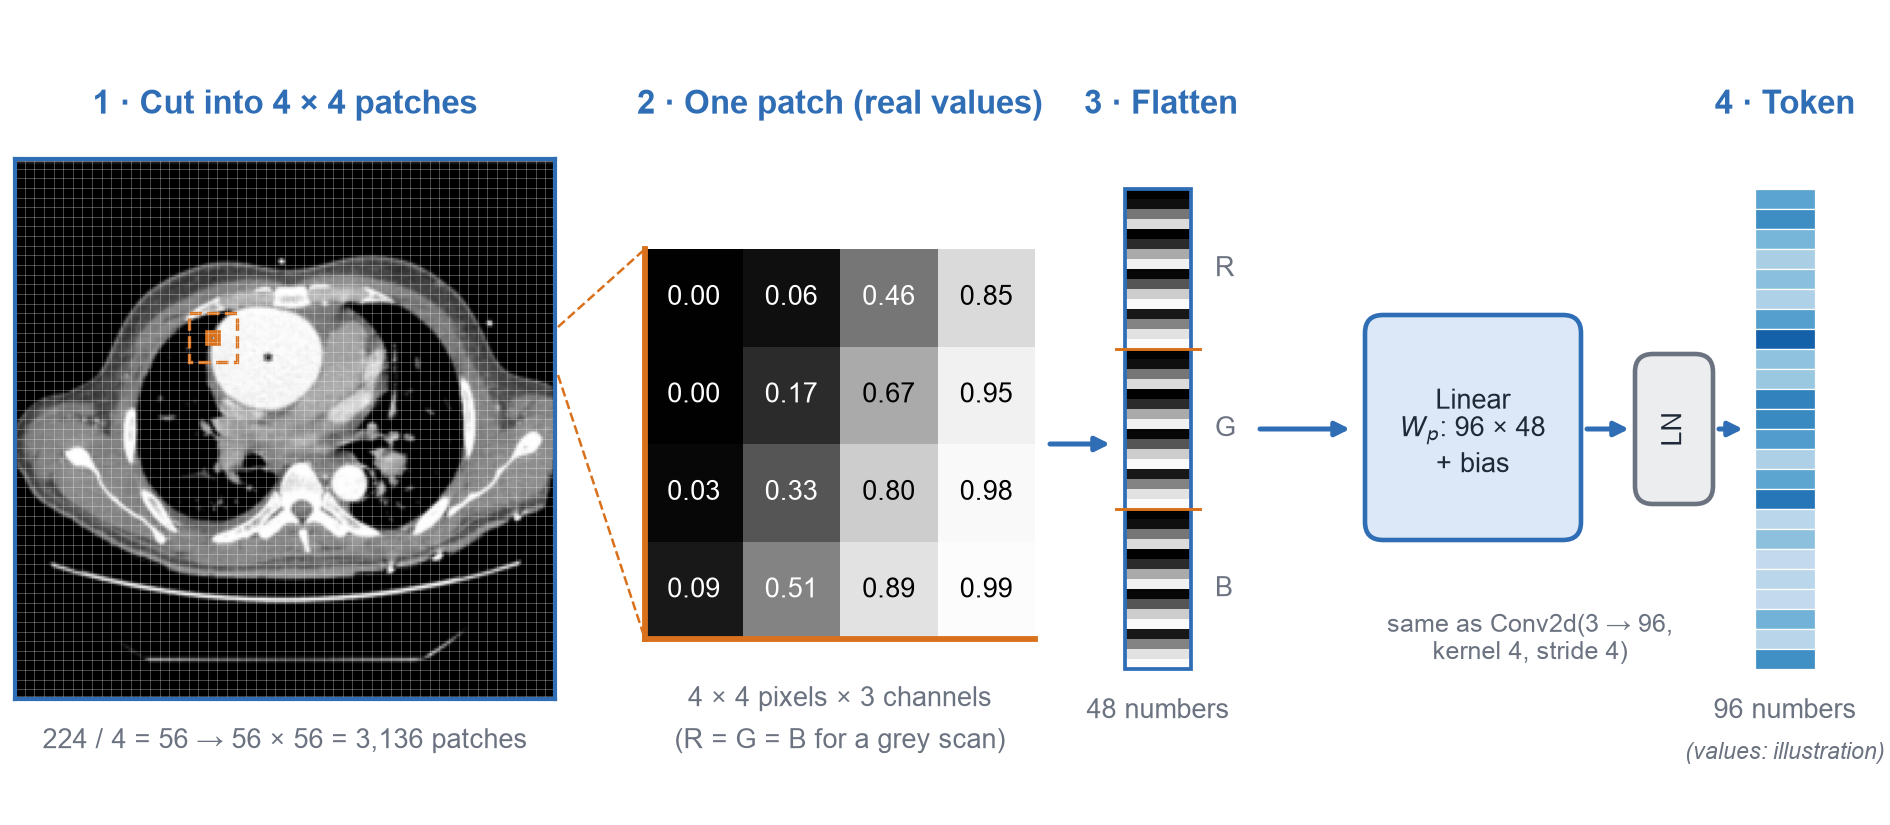
\includegraphics[width=0.92\linewidth,height=\textheight,keepaspectratio]{figures/fig3_4_patch_embed.png}
\caption{Patch embedding pipeline. The $224 \times 224$ radiograph is partitioned into a $56 \times 56$ lattice of $4 \times 4$ patches ($48$ values each), projected linearly to dimension $C=96$, and normalized via LayerNorm.}
\end{figure}

\begin{takeawaybox}
\textbf{DL Architectural Design Choice.} Treating pixels directly as tokens would yield $50{,}176$ sequence positions, inducing an intractable attention memory footprint. Patch partitioning reduces the sequence length by a factor of $P^2 = 16$ ($3{,}136$ tokens) while preserving local sub-anatomical structures.
\end{takeawaybox}

\section{Step 2 --- Swin Transformer Block Architecture}

The token sequence passes through 12 Swin Transformer blocks distributed across 4 stages ($[2, 2, 6, 2]$). Every block employs a pre-LayerNorm (Pre-LN) residual architecture:

\begin{equation}
\hat{z}^{\,l} = \text{W-MSA}\left(\mathrm{LN}\left(z^{\,l-1}\right)\right) + z^{\,l-1}, \qquad z^{\,l} = \mathrm{MLP}\left(\mathrm{LN}\left(\hat{z}^{\,l}\right)\right) + \hat{z}^{\,l} \tag{3.5}
\end{equation}

\begin{equation}
\hat{z}^{\,l+1} = \text{SW-MSA}\left(\mathrm{LN}\left(z^{\,l}\right)\right) + z^{\,l}, \qquad z^{\,l+1} = \mathrm{MLP}\left(\mathrm{LN}\left(\hat{z}^{\,l+1}\right)\right) + \hat{z}^{\,l+1} \tag{3.6}
\end{equation}

where $\text{W-MSA}$ denotes Window-based Multi-Head Self-Attention and $\text{SW-MSA}$ denotes Shifted-Window Multi-Head Self-Attention.

\begin{figure}[!htbp]
\centering
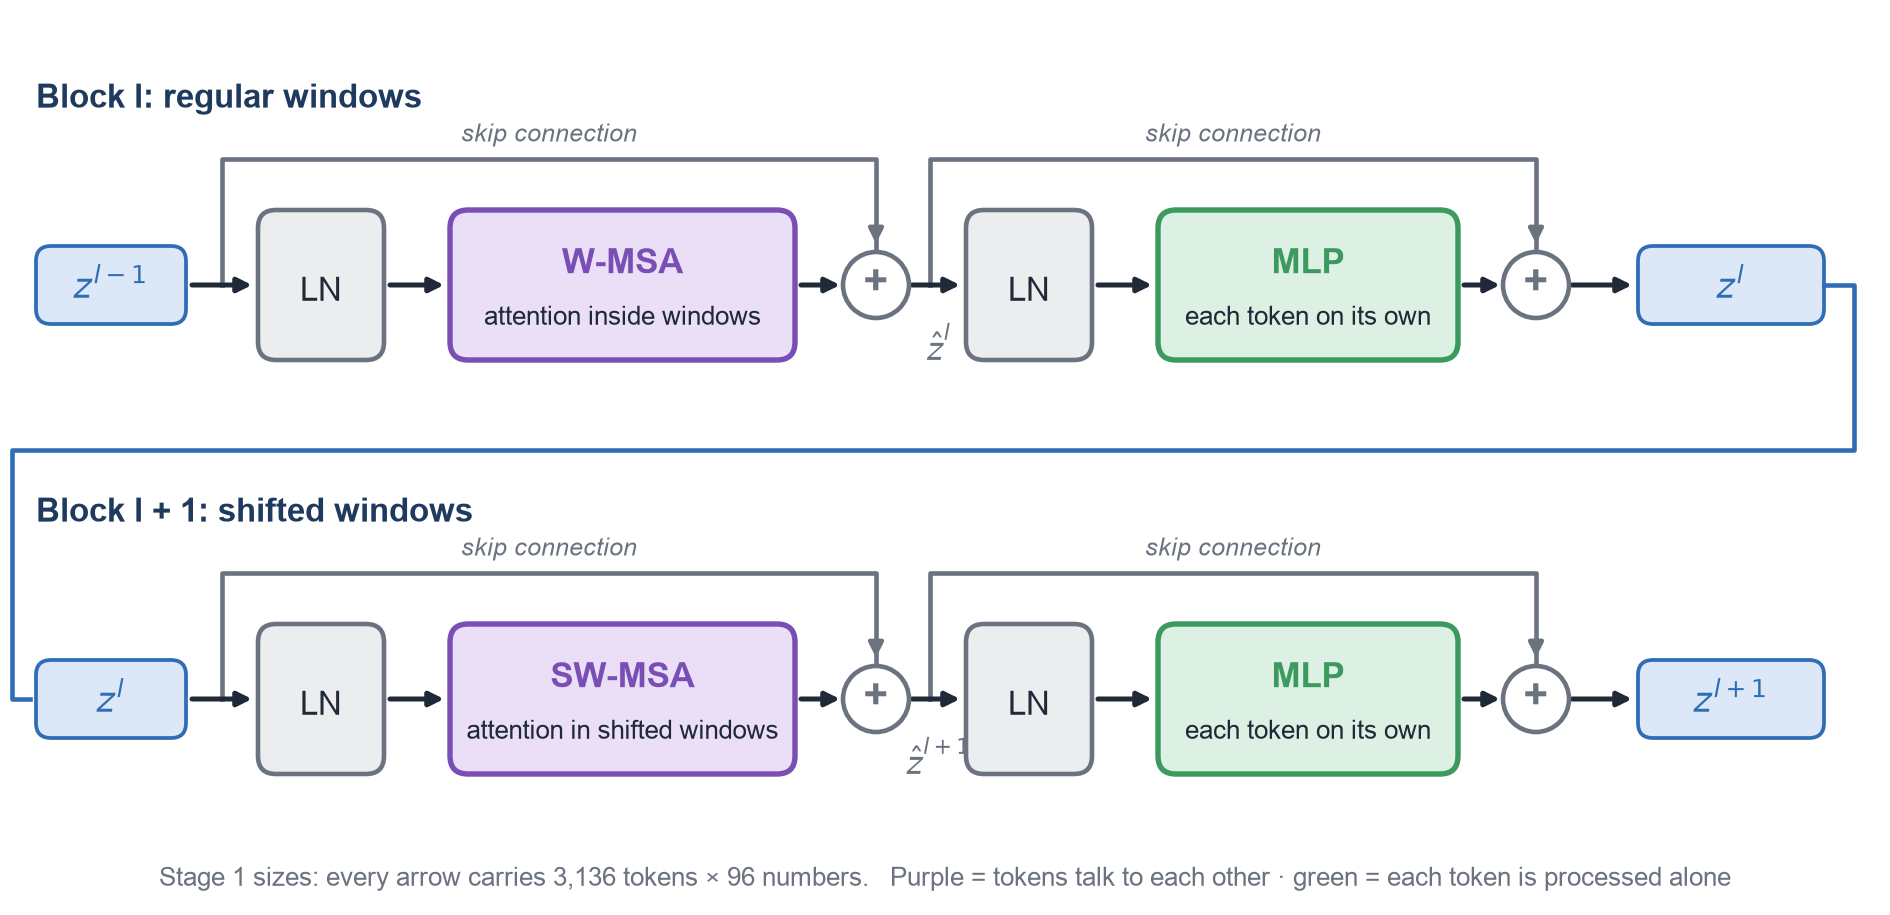
\includegraphics[width=0.88\linewidth,height=\textheight,keepaspectratio]{figures/fig3_9_block.png}
\caption{Consecutive Swin Transformer block pair. Block $l$ applies local window self-attention (W-MSA), and block $l+1$ applies shifted-window self-attention (SW-MSA). Both utilize pre-LayerNorm and residual skip connections.}
\end{figure}

\textbf{Sub-Layer Components:}
\begin{itemize}
\item \textbf{Layer Normalization (LN):} Normalizes activations across channel dimensions independently per token, ensuring numerical stability across deep feature hierarchies:
\begin{equation}
\mathrm{LN}(x)_i = \gamma_i \frac{x_i - \mu}{\sqrt{\sigma^2 + \epsilon}} + \beta_i \tag{3.7}
\end{equation}
\item \textbf{Multilayer Perceptron (MLP):} Applies two affine transformations with an intermediate GELU activation, expanding feature width by an expansion ratio of 4 ($C \to 4C \to C$):
\begin{equation}
\mathrm{MLP}(x) = W_2\, \mathrm{GELU}(W_1 x + b_1) + b_2, \qquad W_1 \in \mathbb{R}^{4C \times C}, \quad W_2 \in \mathbb{R}^{C \times 4C} \tag{3.8}
\end{equation}
\item \textbf{Stochastic Depth (DropPath):} Linearly escalates drop probability ($0 \to 0.20$) across blocks, randomly bypassing residual branches during training to act as an implicit ensemble regularizer.
\end{itemize}

\begin{figure}[!htbp]
\centering
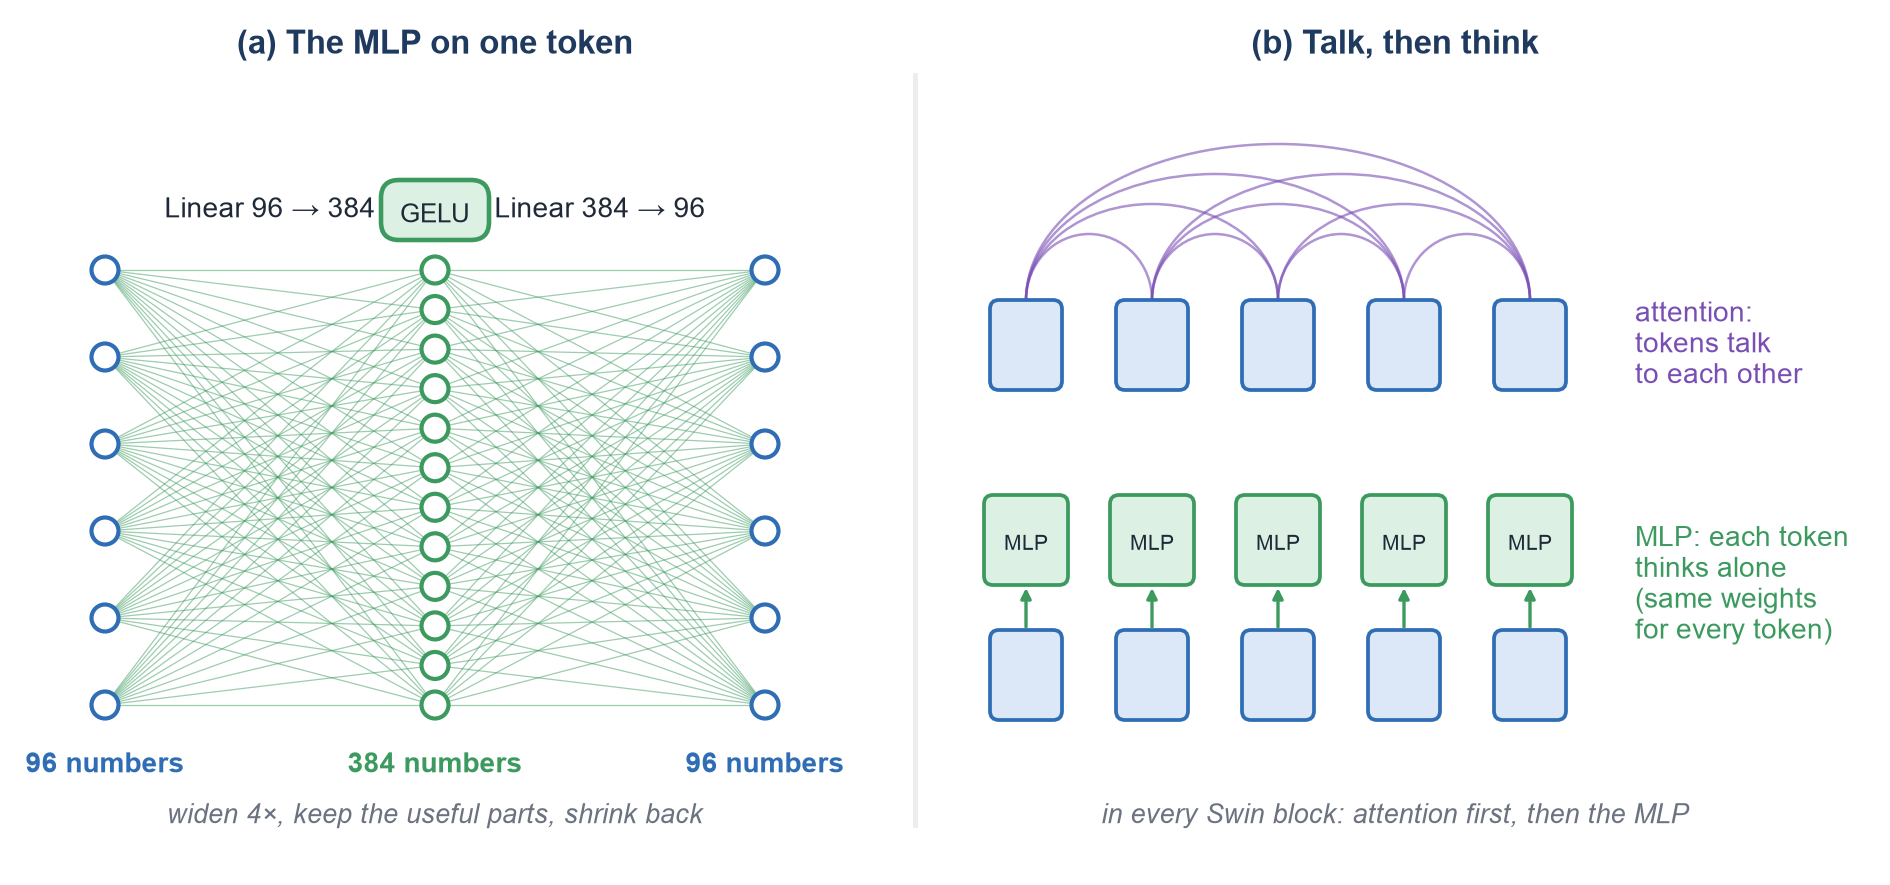
\includegraphics[width=0.88\linewidth,height=\textheight,keepaspectratio]{figures/fig3_15_mlp.png}
\caption{Position-wise Feed-Forward Network (MLP): (a) Expands channel capacity by $4\times$ ($96 \to 384$) before non-linear projection via GELU. (b) Executes independently per spatial token.}
\end{figure}

\section{Step 3 --- Window Attention (W-MSA) and Complexity}

\textbf{Local Window Partitioning.} Standard global Vision Transformer attention scales quadratically with sequence length ($\mathcal{O}(N^2)$), rendering high-resolution medical imaging computationally prohibitive. Swin Transformer resolves this by partitioning the $H \times W$ token lattice into non-overlapping windows of size $M \times M$ ($M = 7$). At Stage 1, this creates $\frac{56}{7} \times \frac{56}{7} = 64$ distinct windows, each containing $M^2 = 49$ tokens.

Self-attention is executed strictly within each window:

\begin{equation}
\text{Attention}(Q, K, V) = \mathrm{softmax}\left(\frac{Q K^\top}{\sqrt{d_k}} + B\right) V \tag{3.9}
\end{equation}

where $Q, K, V \in \mathbb{R}^{M^2 \times d_k}$ and $B \in \mathbb{R}^{M^2 \times M^2}$ is a learned \textbf{continuous relative position bias}. Since spatial coordinates within an $M \times M$ window vary in range $[-M+1, M-1]$, bias values are dynamically indexed from a compact parameter table $\hat{B} \in \mathbb{R}^{(2M-1) \times (2M-1)}$:

\begin{equation}
B_{ij} = \hat{B}\left[\Delta r_{ij} + M - 1,\ \Delta c_{ij} + M - 1\right]
\end{equation}

\textbf{Computational Complexity Comparison.} For a feature map of $h \times w$ patches with $C$ channels:
\begin{equation}
\Omega(\text{Global MSA}) = 4hwC^2 + 2(hw)^2C, \qquad \Omega(\text{W-MSA}) = 4hwC^2 + 2M^2hwC \tag{3.10}
\end{equation}

Because $M = 7$ is fixed, W-MSA scales \textbf{linearly} with image area $hw$. At Stage 1 ($56 \times 56, C=96$), W-MSA requires $\approx 0.15$ GFLOPs compared to $\approx 2.00$ GFLOPs for global attention---a $13.3\times$ computational saving.

\begin{figure}[!htbp]
\centering
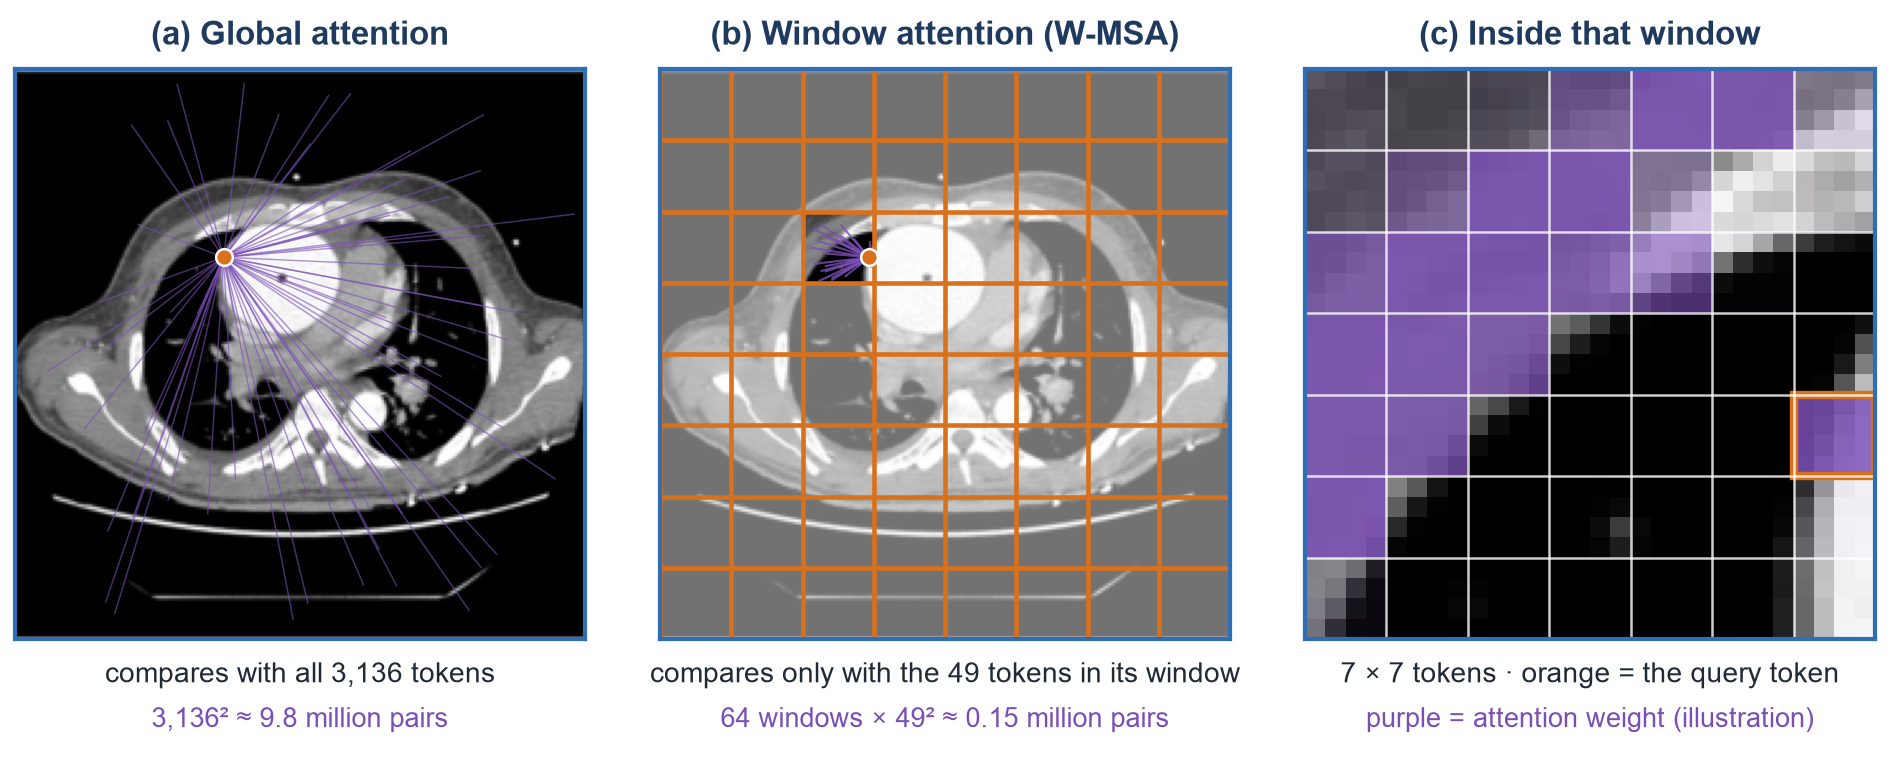
\includegraphics[width=0.92\linewidth,height=\textheight,keepaspectratio]{figures/fig3_11_wmsa.png}
\caption{Comparison of global attention vs.\ local Window-based attention (W-MSA). W-MSA confines pairwise token interactions to $7 \times 7$ spatial windows, bounding quadratic scaling.}
\end{figure}

\section{Step 4 --- Shifted Window Attention (SW-MSA) and Cyclic Shifting}

\textbf{Cross-Window Information Flow.} While W-MSA achieves linear complexity, restricting attention inside static windows eliminates inter-window receptive field growth. To restore cross-window connections without incurring global quadratic cost, consecutive blocks shift the partitioning grid by $\lfloor M/2 \rfloor = 3$ tokens along both spatial axes.

\begin{figure}[!htbp]
\centering
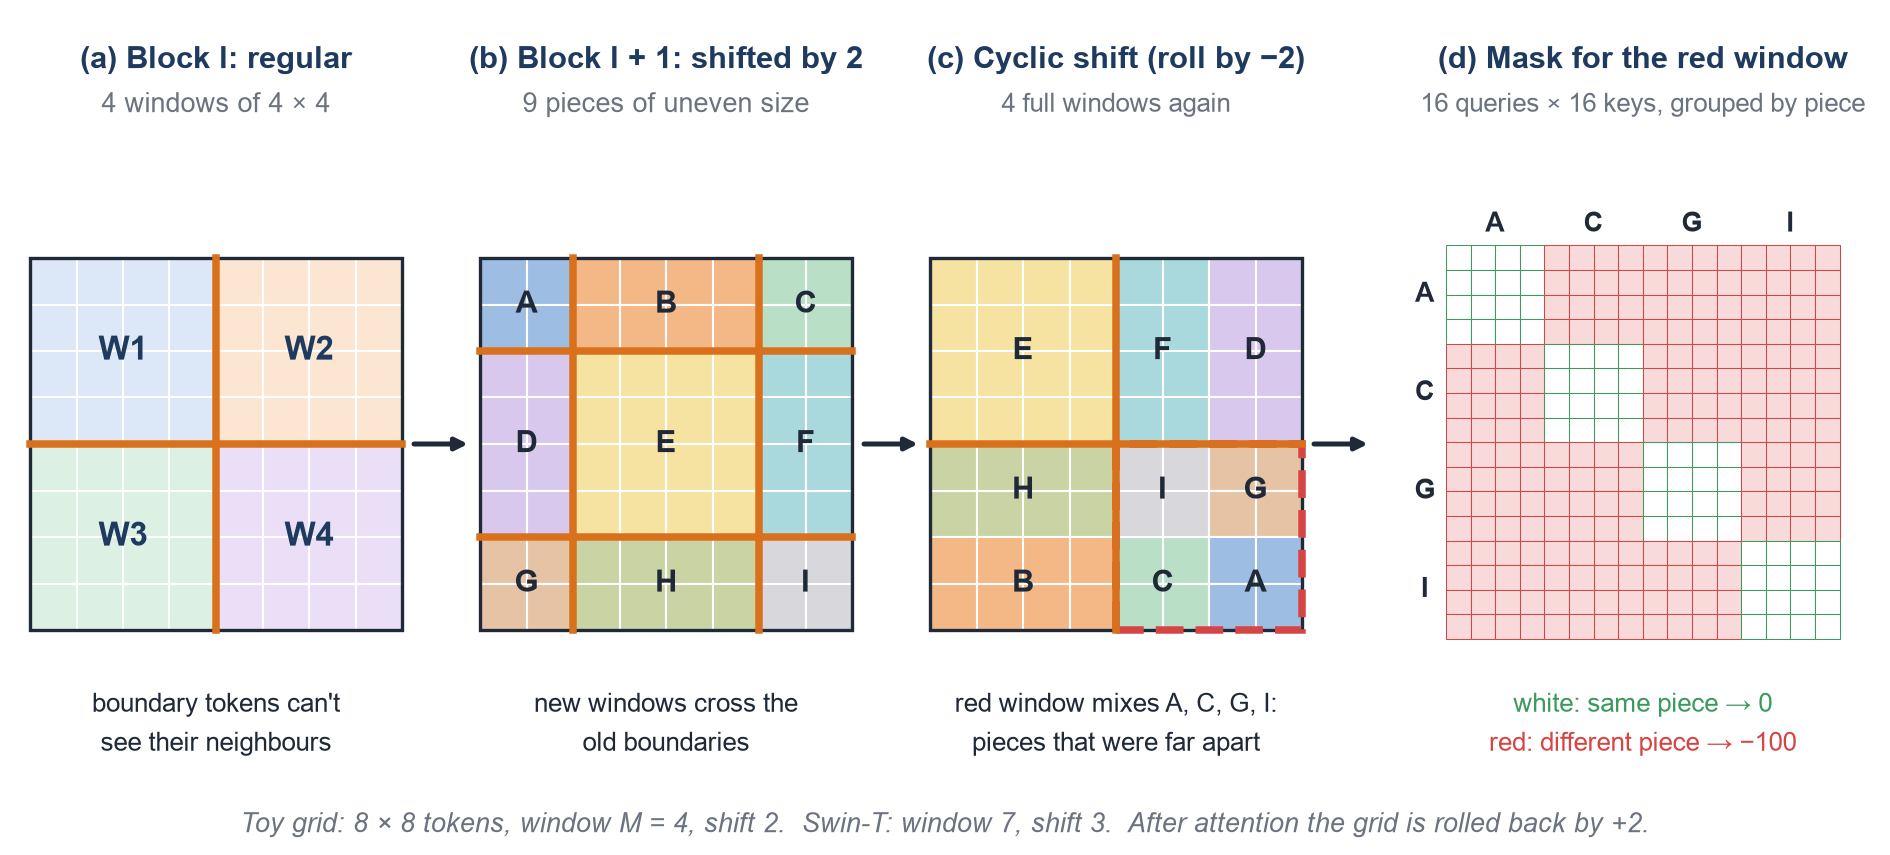
\includegraphics[width=0.90\linewidth,height=\textheight,keepaspectratio]{figures/fig3_17_shift_toy.png}
\caption{Efficient shifted-window computation via cyclic rolling and attention masking. (a) Standard window partition. (b) Shifted windows create sub-window fragments. (c) Cyclic shift merges fragments into regular $M \times M$ windows. (d) Self-attention masking blocks cross-fragment attention.}
\end{figure}

\textbf{Cyclic Shift Formulation.} A naive shift produces $2 \times 2 = 4$ window fragments at borders and corners, increasing the window count from $\lceil \frac{h}{M} \rceil \times \lceil \frac{w}{M} \rceil$ to $(\lceil \frac{h}{M} \rceil + 1) \times (\lceil \frac{w}{M} \rceil + 1)$. Swin Transformer avoids this via \textbf{cyclic rolling}:

\begin{equation}
X'[r, c] = X\left[(r + \lfloor M/2 \rfloor) \bmod H,\ (c + \lfloor M/2 \rfloor) \bmod W\right] \tag{3.11}
\end{equation}

After cyclic shifting, batched window attention is executed with an additive attention mask $\Phi$:

\begin{equation}
\text{SW-MSA} = \mathrm{softmax}\left(\frac{Q K^\top}{\sqrt{d_k}} + B + \Phi\right)V, \qquad \Phi_{ij} = \begin{cases} 0, & \text{tokens } i, j \text{ from same source region} \\ -\infty, & \text{tokens } i, j \text{ from disparate regions} \end{cases} \tag{3.12}
\end{equation}

After attention, a reverse cyclic shift restores tokens to their original geometric positions.

\begin{figure}[!htbp]
\centering
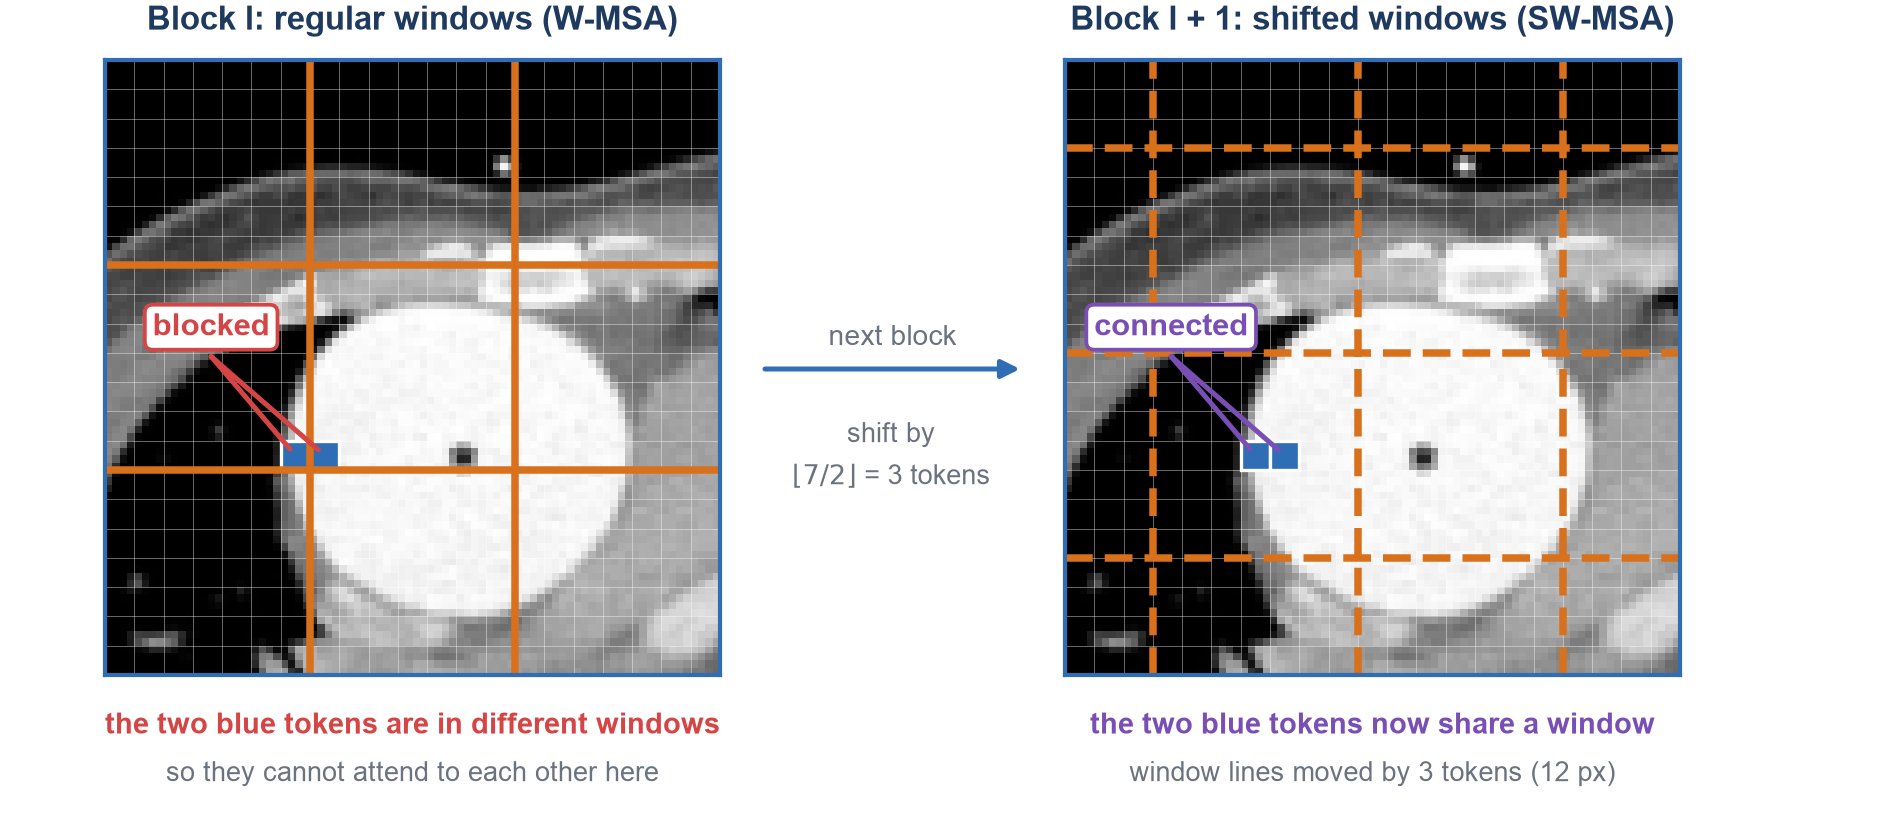
\includegraphics[width=0.82\linewidth,height=\textheight,keepaspectratio]{figures/fig3_18_shift_scan.png}
\caption{Shifted-window receptive field bridging across consecutive blocks on an anatomical scan. Tokens belonging to adjacent partitions in block $l$ share joint attention in block $l+1$.}
\end{figure}

\section{Step 5 --- Hierarchical Patch Merging and Image Memory}

\textbf{Spatial Downsampling and Channel Expansion.} To construct a multiscale feature pyramid analogous to a CNN, \textbf{Patch Merging} layers are inserted between stages. Each patch merging layer concatenates $2 \times 2$ spatially neighboring tokens ($4C$ channels), normalizes them via LayerNorm, and applies a linear projection to reduce channels to $2C$:

\begin{equation}
z'_{ij} = W_m\, \mathrm{LN}\left(\left[x_{2i,2j} \,\|\, x_{2i+1,2j} \,\|\, x_{2i,2j+1} \,\|\, x_{2i+1,2j+1}\right]\right), \qquad W_m \in \mathbb{R}^{2C \times 4C} \tag{3.13}
\end{equation}

This operation halves spatial resolution while doubling channel capacity across the 4 hierarchy stages (Table 3.1).

\begin{figure}[!htbp]
\centering
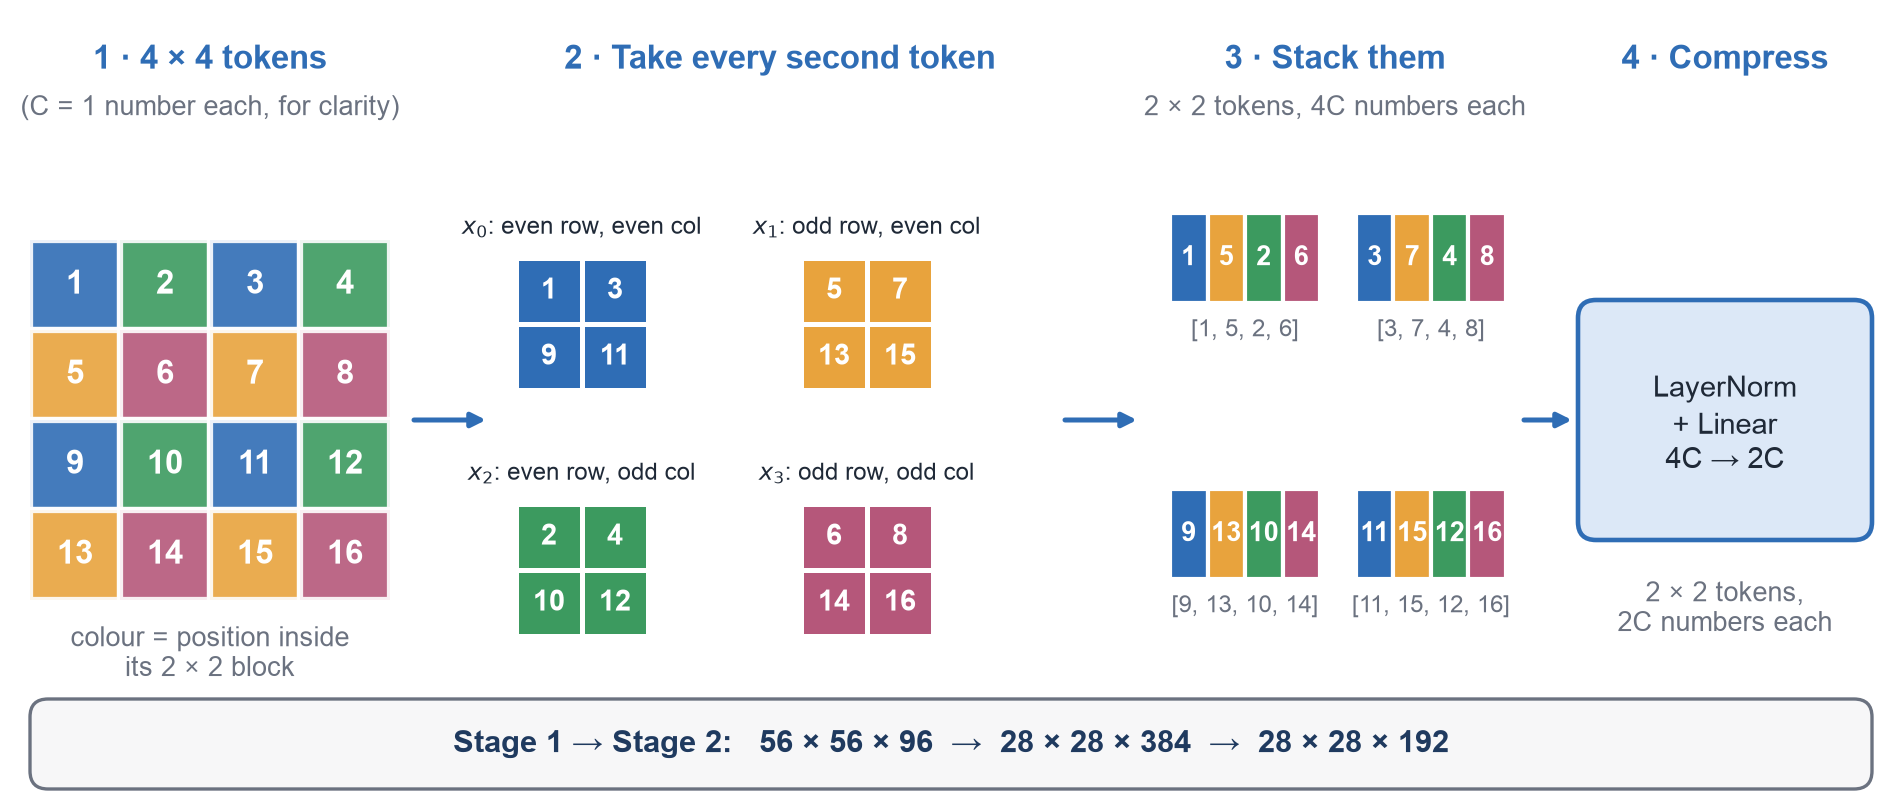
\includegraphics[width=0.92\linewidth,height=\textheight,keepaspectratio]{figures/fig3_5_merge.png}
\caption{Patch Merging operation. Spatial tokens within each $2 \times 2$ neighborhood are concatenated ($4C$ channels) and linearly projected to $2C$, reducing spatial dimension by $2\times$.}
\end{figure}

\needspace{14\baselineskip}

\begin{table}[!htbp]
\centering
\small
\caption{Architectural parameters across the four hierarchical stages of Swin-T.}
\begin{tabular}{@{}ccccccc@{}}
\toprule
\textbf{Stage} & \textbf{Spatial Lattice} & \textbf{Channels ($C$)} & \textbf{Blocks} & \textbf{Heads} & \textbf{Windows ($n_W$)} & \textbf{Patch Field} \\
\midrule
1 & $56 \times 56$ & 96 & 2 & 3 & 64 & $4 \times 4$ px \\
2 & $28 \times 28$ & 192 & 2 & 6 & 16 & $8 \times 8$ px \\
3 & $14 \times 14$ & 384 & 6 & 12 & 4 & $16 \times 16$ px \\
4 & $7 \times 7$ & 768 & 2 & 24 & 1 & $32 \times 32$ px \\
\bottomrule
\end{tabular}
\end{table}

\textbf{Extraction of the Spatial Image Memory ($Z$).}
Following Stage 4 and a final LayerNorm, the resulting feature map of shape $B \times 7 \times 7 \times 768$ is flattened along its spatial dimensions into the \textbf{Visual Memory Tensor}:

\begin{equation}
Z = \mathrm{flatten}_{1,2}\left(\mathrm{LN}\left(\mathrm{SwinStage}_4(X)\right)\right) \in \mathbb{R}^{B \times 49 \times 768}
\end{equation}

Unlike classical CNN architectures that collapse spatial dimensionality via global average pooling ($\mathbb{R}^{B \times 2048} \to \mathbb{R}^{B \times 512}$), our pipeline preserves all \textbf{49 spatial visual memory tokens}. This directly empowers the subsequent language decoder to selectively attend to localized radiographic findings via multi-head cross-attention.

\begin{figure}[!htbp]
\centering
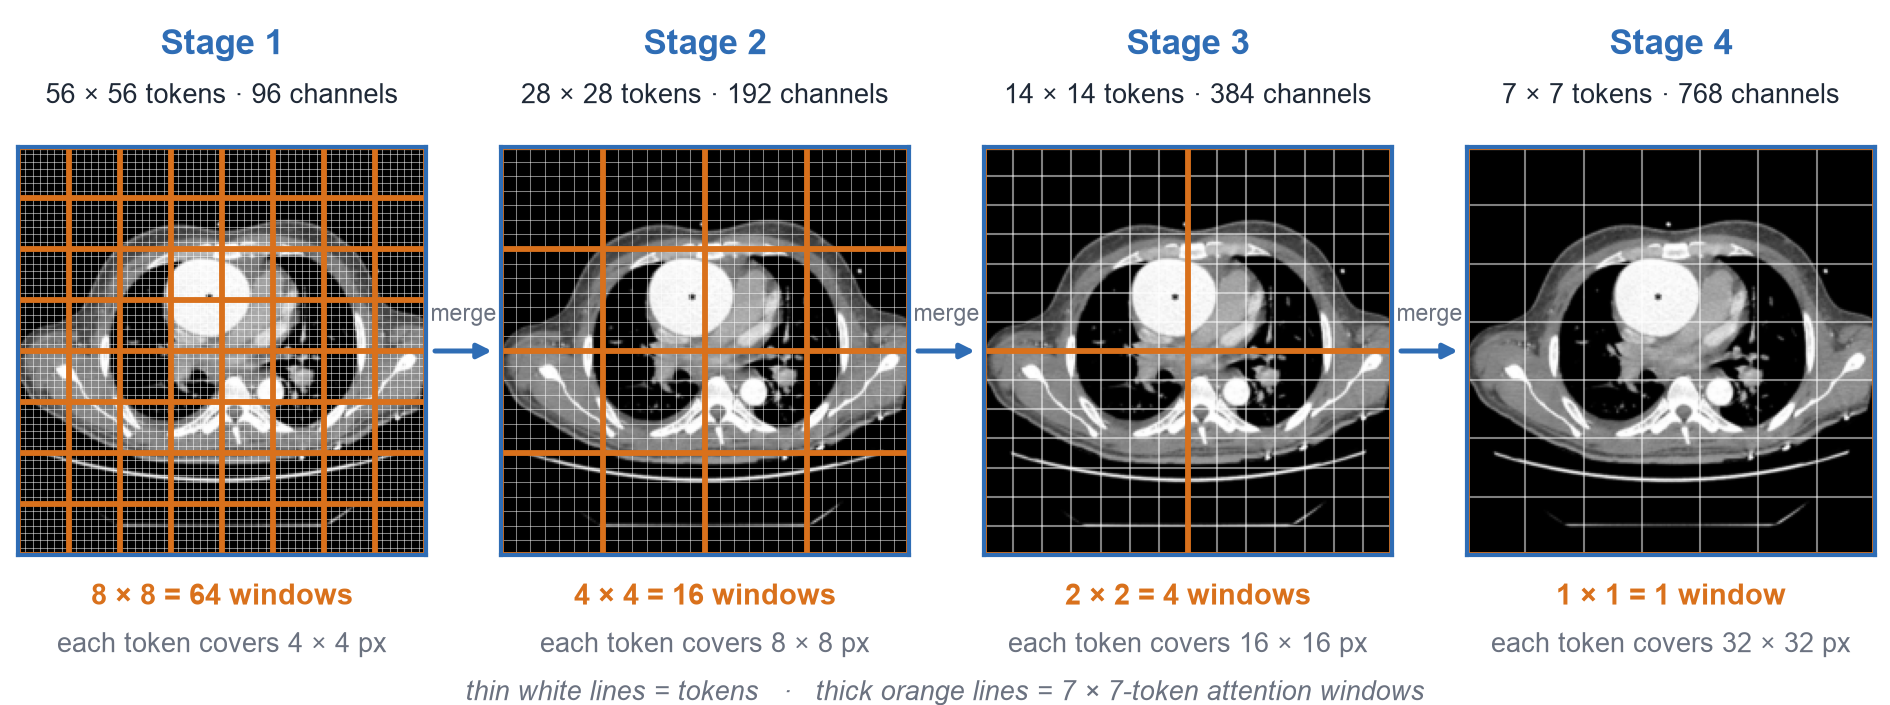
\includegraphics[width=0.94\linewidth,height=\textheight,keepaspectratio]{figures/fig3_6_journey.png}
\caption{Progression of spatial representations through Stages 1--4. Fine boundary features in Stage 1 ($56 \times 56$) hierarchically aggregate into semantically dense diagnostic tokens in Stage 4 ($7 \times 7 \times 768$).}
\end{figure}
